\documentclass[3p]{elsarticle} %preprint/3p

\usepackage{hyperref}

\journal{   }

\usepackage{amsmath} %added for maths environments (equation and align)
\usepackage{amssymb}
\usepackage{upgreek}
\usepackage{bm} %bold symbols by using \bm
\usepackage{mathtools, nccmath} %added for \xrightleftharpoons
\usepackage{stmaryrd} %math symbols
\usepackage{subcaption} %allowing for subcaptions and subfigures
\captionsetup[sub]{font=normalsize}%normalsize

\usepackage{algorithm} %added for algorithm box
\usepackage{algpseudocode}
\biboptions{sort&compress}

\usepackage[autostyle]{csquotes}
\MakeOuterQuote{"}

\bibliographystyle{elsarticle-num}

% slightly altering rules for figure placement to prevent full-page figures
\usepackage{placeins}
\renewcommand{\floatpagefraction}{.90}
\renewcommand{\topfraction}{.90}

\usepackage[capitalise, nameinlink]{cleveref}

\usepackage{todonotes} %added for todo notes
\let\oldtodo\todo
\renewcommand{\todo}[1]{\oldtodo[inline]{#1}}
%\renewcommand{\todo}[1]{\oldtodo[color=white!40,inline]{#1}}
\newcommand{\toask}[1]{\oldtodo[color=green!40, inline]{#1}}
\newcommand{\wrn}[1]{\oldtodo[color=red!40, inline]{#1}}

\usepackage{xcolor}
\usepackage{listings}
\usepackage{lstautogobble}
\usepackage[numbered]{matlab-prettifier}
\lstdefinestyle{mystyle}{
	numbers=left,
	numberstyle=\footnotesize,
	numbersep=8pt,
	style=Matlab-editor,
	tabsize=4,
	basicstyle=\ttfamily\footnotesize,
	numbersep=12pt,
	frame=none,
	autogobble=true
}

\newcommand{\citeMe}{\href{https://doi.org/10.1016/j.cma.2023.116235}{T Hageman, JZ Mejia, R Duddu, and E {Martinez-Pa{\~n}eda}. \textit{Ice Viscosity Governs Hydraulic Fracture Causing Rapid Drainage of Supraglacial Lakes}. The Cryosphere} \citep{Hageman}}

\begin{document}
\pagenumbering{gobble}
\begin{frontmatter}
\title{IceHydroFrac: A MATLAB code to simulate water-filled crevasse propagation and uplifting of ice sheets }

\author[1]{Tim Hageman \corref{mycorrespondingauthor}}
\cortext[mycorrespondingauthor]{Corresponding author}
\ead{tim.hageman@eng.ox.ac.uk}
\author[2]{Jessica Mejía}
\author[3]{Ravindra Duddu} 
\author[1]{Emilio Martínez-Pañeda}

\address[1]{Department of Engineering Science, University of Oxford, Oxford OX1 3PJ, UK}
\address[2]{Department of Geology, University at Buffalo, Buffalo, NY 14260, USA}
\address[3]{Department of Civil and Environmental Engineering, Department of Earth and Environmental Sciences, Vanderbilt University, Nashville, TN 37235, USA}

\begin{abstract}
Documentation that accompanies the \textit{MATLAB} code \href{https://github.com/T-Hageman/MATLAB_IceHydroFrac}{IceHydroFrac, available from \textcolor{blue}{here}}. This documentation explains the usage of the implemented finite element framework, and highlight the main files.  The code allows the simulation of a single propagating crevasse through an ice-sheet, driven by a surface lake. Upon reaching the base, sideways cracks are included, allowing the subsequent uplifting to be captured. As the code allows for both visco-plastic and linear-elastic rheologies, it has been used to demonstrate the importance of including viscous effects, even on the relatively short time-scales involved with fracture propagation. As thermal effects are also included, an in-depth look at the effects of melting/freezing, thermal conduction of heat into the ice, and frictional heating within the crevasse is made possible. For further findings, see the main paper at \citeMe{}. 

If using this module, please cite: \citeMe{}.
\end{abstract}

\begin{keyword}
MATLAB, Hydraulic fracture, Greenland Ice Sheet, Crevasse, Numerical simulation, Viscous effects
\end{keyword}

\end{frontmatter}

\begin{figure}
	\centering
	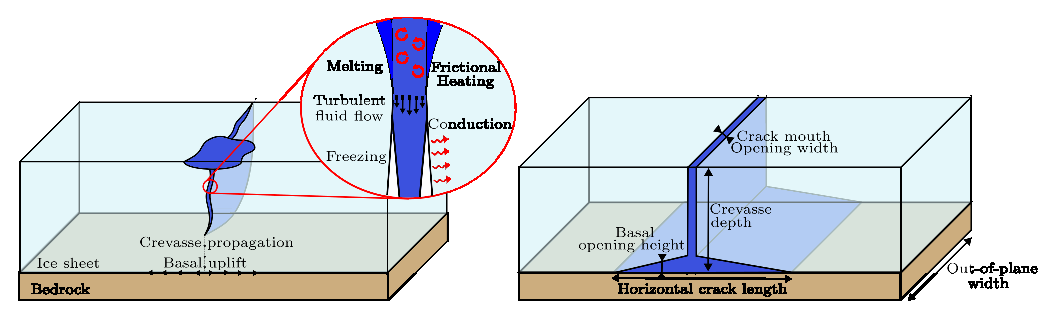
\includegraphics[width=16cm]{Figures/CaseOverview.eps}
	\caption{Overview of the system simulated using the presented MATLAB code}
\end{figure}

\newpage
\tableofcontents

\newpage
\pagenumbering{arabic}
\section{Introduction}
Water-driven crevasses can have a large impact on the overall behaviour of ice-sheets \citep{Boon2003,Phillips2010a,Poinar2021,Krawczynski2009}. They transfer water to the bed, reducing friction at the base and accelerating ice flow \citep{Fountain2005,Smith2015,Dow2015}. Furthermore, they have the potential to cause premature ice-cliff collapses \citep{Scambos2009,McGrath2012,Buck2023}. However, these crevasses are complicated to capture through computational modelling, due to the range of length-scales involved within the cracking process \citep{Rice2015}. Additional effects due to thermal energy produced by friction, and lost due to conduction into the ice, further complicate the modelling as the resulting melting will alter the crack opening \citep{Andrews2022}, and can potentially halt the propagation due to freezing. 

Here, we describe a finite element model capable of simulating hydro-fracture through linear-elastic and visco-plastic ice. This model uses interface elements to represent the crack path, and through a two-scale description allows for accurately capturing the phenomena surrounding crevasse propagation. The MATLAB code has been used and verified to work in MATLAB versions 2023b and 2022b, with earlier versions also potentially compatible (but not verified). In the remainder of this documentation, the basic usage of this code will be discussed in \cref{sec:usage}, after which \cref{sec:models} will explain the individual components used to represent the physics relevant to ice sheet hydro-fracture. Finally, in \cref{sec:postprocessing} the resulting output files are discussed, and the post-processing procedures are explained. 

For a more detailed description of the results from this model, and a discussion on the relevance of including thermals and using a visco-plastic rheology, see \citeMe{}.

\subsection{Basic usage}
\label{sec:usage}
All parameters are set within and relevant functions are called from the matlab file "main.m", and running this file performs the full simulation. Parameters are also set within this file, for instance defining the visco-plastic model through:
\lstinputlisting[firstnumber=64,firstline=64,lastline=73,style=mystyle,title=main.m]{../main.m}
These parameters are automatically passed along to the relevant physics models once they are initialized. As such, no changes in other files are needed to adapt the simulation set-up for other parameters. 

\section{Summary of included files}
The code is set up in a object-oriented manner, defining matlab classes for each sub-component and providing their accompanying methods. As a result, a clear distinction is made between different components, and each can be used and altered with limited/no impact on other components. Here, the different classes are described. The commenting style employed within the code is compatible with the matlab help function, as such information about all usable methods within a class can be accessed by including the relevant folders, and typing, for instance, "help Solver" to print all variables contained within and all function available from the solver. 

\subsection{main.m}
This is the main file, from which all classes are constructed and the actual simulation is performed. Within it, all properties used within other classes are defined as inputs. These properties are then passed on to initialize the "physics" object, via 
\lstinputlisting[firstnumber=147,firstline=147,lastline=148,style=mystyle,title=main.m]{../main.m}
taking all relevant input parameters within the physics\_ in structure, and an initial time step increment dt0. In a similar manner, the mesh is also initialized from a structure of properties, 
\lstinputlisting[firstnumber=142,firstline=142,lastline=145,style=mystyle]{../main.m}
which reads the mesh from a file, initializes the required elements and node groups, displays the mesh in  a figure, and confirms the mesh is valid and prints statistics related to the area of each separate element group to the output. Finally, the main file performs the time-stepping, calling the function:
\lstinputlisting[firstnumber=195,firstline=195,lastline=196,style=mystyle]{../main.m}
to solve the actual time increments. 

After each time increment, outputs are saved into a single structure for later plotting, 
\lstinputlisting[firstnumber=198,firstline=198,lastline=208,style=mystyle]{../main.m}
These outputs are:
\begin{enumerate}
  \setcounter{enumi}{199}
  \item tvec: This contains all time increments at which the other elements within this structure have outputted data. Notably, as the time increment varies between the initialization period ($tvec(i)<0$) and actual simulations ($tvec(i)\geq 0$) differs, this vector is also required to translate the number of the time step (as used within the naming of full output files) to the actual time of the outputs.
  \item Lfrac: This is the length all fractured interfaces. When the crevasse has yet to reach the base, this corresponds to the depth of the crevasse. After reaching the bottom, this is the depth of the crevasse (=the ice thickness) plus the total length of the horizontal cracks (both directions summed together).
  \item Qvec: This reports the total thermal energies produced/consumed throughout the simulation. The first element of this vector corresponds to the thermal energy conducted into the ice, the second to the heat produced by the turbulent flow due to friction, and the final element corresponds to the thermal energy used to cause freezing/melting of the crevasse walls. These values are the integrated totals for the complete crack, and are also integrated over the complete time. 
  \item Qinflow: The total volume of fluid that has entered the crevasse from the inlet at the surface. As with all other outputs, this is given per metre of unit depth.  
  \item qCurrent: The current fluid inflow at the top inlet, $\partial \text{Qinflow}/\partial t$.
  \item upLift: Surface displacement at the centre of the top surface, coinciding with the crevasse. This contains the horizontal displacement (half the crevasse opening height), and the vertical displacement.
  \setcounter{enumi}{206}
  \item SurfaceDisp: Vectors containing horizontal and vertical displacements for the complete top surface of the ice-sheet. The coordinates that correspond to the given data points are saved within TimeSeries.SurfaceCoords. 
\end{enumerate}
In addition to these time series, full outputs are saved after every 10 time steps, 
\lstinputlisting[firstnumber=215,firstline=215,lastline=219,style=mystyle]{../main.m}
These output files are appended with the number of the time increment during which the output is saved, and they contain all information required to restart a previously interrupted simulation. 

\subsection{Models}
\label{sec:models}
The models implement parts of the relevant physics. At initialization time, models are constructed by passing their relevant input parameters as:
\lstinputlisting[firstnumber=47,firstline=47,lastline=47,style=mystyle,title=Models/@ViscoElastic/ViscoElastic.m]{../Models/@ViscoElastic/ViscoElastic.m}
This also saves pointers to the physics and mesh objects, allowing interacting with these whenever needed. The physics implemented by the model are added within the GetKf function, called whenever an updated tangent stiffness matrix and/or force vector is needed:
\lstinputlisting[firstnumber=256,firstline=256,lastline=256,style=mystyle]{../Models/@ViscoElastic/ViscoElastic.m}
When models have history-dependent parameters, these are updated by calling the commit function, 
\lstinputlisting[firstnumber=127,firstline=127,lastline=127,style=mystyle]{../Models/@ViscoElastic/ViscoElastic.m}
where the commit type indicates either "TimeDep" for committing time-irreversible data (e.g. plastic strains, time-integrated quantities), "irreversibles" for path-irreversible quantities (e.g. cohesive zone models), and "StartIt" for anything that needs to be performed at the start of each time increment.  


\subsubsection{ViscoElastic.m}
This model implements the static momentum balance:
\begin{equation}
-\nabla \cdot \bm{\sigma} = \bm{0} \label{eq:mom}
\end{equation}
with the weak form of this contribution given by:
\begin{equation}
\int_\Omega \bm{B}^T \bm{D} \bm{B}\bm{u}^{t+\Delta t} - \bm{B}^T \bm{D} \varepsilon_{\text{v}}^{t+\Delta t}\;\text{d}\Omega \label{eq:weak_mom}
\end{equation}
with the plastic strains determined once per time increment using glens law \citep{Glen1955,Weertman1983}, based on the displacements at the end of the previous time increment:
\begin{equation}
	\mathbf{\varepsilon}_{\text{v}}^{t+\Delta t} = \mathbf{\varepsilon}_{\text{v}}^{t}+\Delta t A \left( \left({\mathbf{u}^{t}}^T\bm{B}^T-\mathbf{\varepsilon}_{\text{v}}^{t+\Delta t}\right) \bm{D}^T \bm{J_2}\bm{D} \left(\bm{B} \mathbf{u}^t-\mathbf{\varepsilon}_{\text{v}}^{t+\Delta t}\right) \right)^{\frac{n-1}{2}}\bm{J_2}\bm{D} \left(\bm{B} \mathbf{u}^t-\mathbf{\varepsilon}_{\text{v}}^{t+\Delta t}\right)
\end{equation}
with $\bm{B}$ the displacement to strain mapping matrix, $\epsilon=\bm{B}\mathbf{u}$, and $\bm{J}_2$ the deviatoric stress operator:
\begin{equation}
	\mathbf{\sigma}_{dev} = \bm{J} \mathbf{\sigma} \qquad \bm{J}_2 = \begin{bmatrix} 2/3 & -1/3 & -1/3 & 0\\ -1/3 & -1/3 & 2/3 & 0 \\ -1/3 & -1/3 & 2/3 & 0 \\ 0 & 0 & 0 & 1 \end{bmatrix} 
\end{equation}

The input parameters for this model are defined by:
\lstinputlisting[firstnumber=64,firstline=64,lastline=74,style=mystyle,title=main.m]{../main.m}
where "Type" is the name of this model, "Egroup" indicates the domain this model is applied to, and all other are the physical parameters for this model. The temperature of the ice is defined as an interpolation function, which is previously loaded from a file or defined to return a constant by:
\lstinputlisting[firstnumber=12,firstline=12,lastline=17,style=mystyle]{../main.m}


For computational efficiency, \cref{eq:weak_mom} is split into two contributions: The first term contributes to the stiffness matrix and force vector, with the stiffness matrix only needing to be updated when the mesh changes (due to crack propagation):
\lstinputlisting[firstnumber=263,firstline=263,lastline=267,style=mystyle,title=Models/@ViscoElastic/ViscoElastic.m]{../Models/@ViscoElastic/ViscoElastic.m}
, with the stiffness matrix assembled in a standard manner as:
\lstinputlisting[firstnumber=286,firstline=286,lastline=290,style=mystyle]{../Models/@ViscoElastic/ViscoElastic.m}
where the height of integration points is checked to determine whether elements are located within the ice or rock parts of the domain. This tangent matrix is then used together with a similar force vector resulting for the viscous part of \cref{eq:weak_mom} to add contributions to the global foce vector as:
\lstinputlisting[firstnumber=300,firstline=300,lastline=304,style=mystyle]{../Models/@ViscoElastic/ViscoElastic.m}
As a result, the force vector for the visco-plastic component and the tangent matrix for the linear-elastic components only need to be updated once per time increment, independent of the actual amount of non-linear iterations performed within that increment.

\subsubsection{Inertia.m}
This model adds inertia terms to the momentum balance, appending the momentum balance from \cref{eq:mom} to read:
\begin{equation}
	\rho_\pi \ddot{\mathbf{u}} - \nabla \cdot \mathbf{\sigma} = \mathbf{0}
\end{equation}
where the first term is the newly added term in this model (note: this model is additive to the ViscoElastic.m model, it does not add the stress term by itself). The inputs required to initialize this model are given by:
\lstinputlisting[firstnumber=76,firstline=76,lastline=81,style=mystyle,title=main.m]{../main.m}
where the time discretisation parameters beta and gamma are used to define the acceleration in terms of history parameters (the old velocity and acceleration) and the current displacement as:
\begin{align}
     \dot{\mathbf{u}}^{t+\Delta t} &= \frac{\gamma}{\beta \Delta t} \left(\mathbf{u}^{t+\Delta t} - \mathbf{u}^t \right) - \left( \frac{\gamma}{\beta} - 1\right) \dot{\mathbf{u}}^t - \left(\frac{\Delta t \gamma}{2\beta} - \Delta t\right) \ddot{\mathbf{u}}^t \\
    \ddot{\mathbf{u}}^{t+\Delta t} &= \frac{1}{\beta \Delta t^2}  \left(\mathbf{u}^{t+\Delta t} - \mathbf{u}^t \right) - \frac{1}{\beta \Delta t} \dot{\mathbf{u}}^t - \left(\frac{1}{2\beta} - 1\right) \ddot{\mathbf{u}}^t 
\end{align}
Similar to the viscoelastic model, the tangent matrix for this model is calculated once, and then re-used to assemble the global tangent matrix every iteration. 

\subsubsection{SelfWeight.m}
This model adds the gravity contribution to the momentum balance, appending the momentum balance to:
\begin{equation}
	\rho_\pi \ddot{\mathbf{u}} - \nabla \cdot \mathbf{\sigma} - \rho_\pi \mathbf{g}= \mathbf{0}
\end{equation}
For simplicity, this gravity force is added to the global force vector, with no differentiation made between internal and external forces. Inputs for this model are the element group the model is acting on, and the densities of ice and rock:
\lstinputlisting[firstnumber=83,firstline=83,lastline=87,style=mystyle,title=main.m]{../main.m}

\subsubsection{FractureCZM.m}
This model adds the cohesive fracture model, defined by the interface tractions normal to the fracture surface:
\begin{equation}
    \mathbf{\uptau}_{CZM} = -f_\mathrm{t} \mathbf{n} \exp\left(-\llbracket \mathbf{u} \rrbracket \cdot \mathbf{n} \frac{f_\mathrm{t}}{G_\mathrm{c}}\right)
\end{equation}
It also manages the propagation criteria for fracture propagation, allowing the crack to propagate when $\sigma\cdot \mathbf{n}-f_t>0$. 

To initialize the model, the input parameters required are:
\lstinputlisting[firstnumber=88,firstline=88,lastline=94,style=mystyle,title=main.m]{../main.m}
where the temperature profile that is given as input is used to obtain the tensile strength via:
\lstinputlisting[firstnumber=45,firstline=45,lastline=45,style=mystyle,title=Models/@FractureCZM/FractureCZM.m]{../Models/@FractureCZM/FractureCZM.m}

For the surface tractions, the maximum displacement is saved as a history variable, saved during the assembly of the force and tangent stiffness matrix:
\lstinputlisting[firstnumber=155,firstline=155,lastline=167,style=mystyle]{../Models/@FractureCZM/FractureCZM.m}
which also produces the surface traction normal to the surface, tau(1), and its derivative dtaudh(1,1). The tangent component of this traction is set to zero, and during assembly this vector is rotated from the local to the global coordinate system. To improve the stability of the no-penetration condition, used to enforce contact between the crevasse walls, a lumped integration scheme is used, with sets of nodes contributing on a set-by-set basis to the overall force vector as:
\lstinputlisting[firstnumber=174,firstline=174,lastline=184,style=mystyle]{../Models/@FractureCZM/FractureCZM.m}
with this condition only activating when the crevasse opening height is negative. 

The fracture criterion is evaluated in the function
\lstinputlisting[firstnumber=57,firstline=57,lastline=57,style=mystyle]{../Models/@FractureCZM/FractureCZM.m}
This function queries the elements ahead of the crack tip to obtain its stresses
\lstinputlisting[firstnumber=58,firstline=58,lastline=59,style=mystyle]{../Models/@FractureCZM/FractureCZM.m}
which are compared to the temperature-dependent tensile strength. If the propagation criterion is exceeded, the mesh is addapted to include a newly inserted interface element:
\lstinputlisting[firstnumber=93,firstline=93,lastline=97,style=mystyle]{../Models/@FractureCZM/FractureCZM.m}

\subsubsection{FractureFluid.m}
FractureFluid.m implements all the fluid flow and thermal related equations for the water within the crevasse, and is defined by the input parameters:
\lstinputlisting[firstnumber=96,firstline=96,lastline=109,style=mystyle,title=main.m]{../main.m}
Notably, the input "FlowModel" allows selecting either turbulent flow, based on a friction factor approach via \citep{Gauckler1867, Strickler1981}:
\begin{equation}
    q = -2\rho_{\text{w}}^{-\frac{1}{2}}k_{\text{wall}}^{-\frac{1}{6}}f_0^{-\frac{1}{2}} h^{\frac{5}{3}}\left|\frac{\partial p}{\partial \xi}-\rho_{\text{w}} \mathbf{g} \cdot \mathbf{s}\right|^{-\frac{1}{2}}\left(\frac{\partial p}{\partial \xi}-\rho_{\text{w}} \mathbf{g} \cdot \mathbf{s}\right) \label{eq:qx}
\end{equation}
or laminar flow, using the analytic solution for uni-directional pressure-driven fluid flow between flat plates:
\begin{equation}
	q = \frac{h^3}{12\mu} \left(\frac{\partial p}{\partial \xi}-\rho_{\text{w}} \mathbf{g} \cdot \mathbf{s}\right)
\end{equation}
with this choice of model being set as either "FrictionFactor" for turbulent flow, or "CubicLaw" for laminar flow. This choice is applied to the complete crevasse, and no checking is performed whether the fluid velocity warrants laminar or turbulent flow (based on simulations performed for our paper, the Reynolds number indicates turbulent for our use cases). 

This fluid flux is used within the mass balance \citep{Boone1990, deBorst2017, Hageman2019}:
\begin{equation}
    \frac{\partial q}{\partial \xi} + \dot{h} - \frac{\rho_{\text{i}}}{\rho_{\text{w}}} \dot{h}_{\text{melt}}+ \frac{h}{K_{\text{w}}}\dot{p} = 0 \label{eq:MassBalance}
\end{equation}
which also requires changes in local opening height, and melting rate. These are obtained by solving the coupled system of equations within each integration point:
\begin{align}
    q &= -2\rho_{\text{w}}^{-\frac{1}{2}}k_{\text{wall}}^{-\frac{1}{6}}f_0^{-\frac{1}{2}} h^{\frac{5}{3}}\left|\frac{\partial p}{\partial \xi}-\rho_{\text{w}} \mathbf{g} \cdot \mathbf{s}\right|^{-\frac{1}{2}}\left(\frac{\partial p}{\partial \xi}-\rho_{\text{w}} \mathbf{g} \cdot \mathbf{s}\right) \label{SIeq:qx}\\
    0&=\rho_{\text{i}} \mathcal{L}\dot{h}_{\text{melt}} + \frac{k^{\frac{1}{2}}T_\infty \rho_{\text{i}}^{\frac{1}{2}}c_{\mathrm{p}}^{\frac{1}{2}}}{\pi^{\frac{1}{2}}\left(t-t_0\right)^{\frac{3}{2}}}  + q \left(\frac{\partial p}{\partial \xi}-\rho_{\text{w}} \mathbf{g} \cdot \mathbf{s}\right) \label{SIeq:hmelt}\\
    h &= h_{\text{melt}} + \mathbf{n}\cdot\llbracket \mathbf{u} \rrbracket\label{SIeq:htotal}
\end{align}
Defining the momentum balance of the fluid, thermal balance, and total opening height respectively. This system is solved in a coupled manner, using:
\begin{equation}
    \bm{C}_{ip} \begin{bmatrix} \mathrm{d}{q}_{ip}^{t+\Delta t} \\ \mathrm{d} {h_{\text{melt}}}_{ip}^{t+\Delta t} \\ \mathrm{d} h^{t+\Delta t}_{ip} \end{bmatrix}_{i+1} = - \begin{bmatrix} f_{1,ip} \\ f_{2,ip} \\ f_{3,ip} \end{bmatrix}_i,
\end{equation}
where the integration-point level tangent matrix given by:
\begin{equation}
    \bm{C}_{ip} = \begin{bmatrix} 1 & 0 & \frac{10}{3}\rho_{\text{w}}^{-\frac{1}{2}}k_{\text{wall}}^{-\frac{1}{6}}f_0^{-\frac{1}{2}} {h_{ip}^{t+\Delta t}}^{\frac{2}{3}}\left|\bm{\nabla}\mathbf{N}_\mathrm{f} \mathbf{p}^{t+\Delta t}-\rho_{\text{w}} \mathbf{g} \cdot \mathbf{s}\right|^{-\frac{1}{2}}\left(\bm{\nabla}\mathbf{N}_\mathrm{f} \mathbf{p}^{t+\Delta t}-\rho_{\text{w}} \mathbf{g} \cdot \mathbf{s}\right) \\
    \bm{\nabla}\mathbf{N}_f \mathbf{p}^{t+\Delta t}-\rho_{\text{w}} \mathbf{g} \cdot \mathbf{s} & \frac{\rho_{\text{i}} \mathcal{L}}{\Delta t} & 0 \\
    0 & -1 & 1\end{bmatrix} \label{SIeq:CMat}
\end{equation}
and during the assembly of the tangent system matrix for the global system, consistent tangent matrices are obtained via:
\begin{equation}
\begin{split}
    &\begin{bmatrix} \frac{\partial q}{\partial \mathbf{p}} & \frac{\partial q}{\partial \mathbf{u}} \\ \frac{\partial h_{\text{melt}}}{\partial \mathbf{p}} & \frac{\partial h_{\text{melt}}}{\partial \mathbf{u}} \\ \frac{\partial h}{\partial \mathbf{p}} & \frac{\partial h}{\partial \mathbf{u}} \end{bmatrix} = -\bm{C}^{-1}_{ip} \begin{bmatrix} \rho_{\text{w}}^{-\frac{1}{2}}k_{\text{wall}}^{-\frac{1}{6}}f_0^{-\frac{1}{2}} {h_{ip}^{t+\Delta t}}^{\frac{5}{3}}\left|\bm{\nabla}\mathbf{N}_\mathrm{f} \mathbf{p}^{t+\Delta t}-\rho_{\text{w}} \mathbf{g} \cdot \mathbf{s}\right|^{-\frac{1}{2}} \bm{\nabla} \mathbf{N}_\mathrm{f} & 0 \\ {q}_{ip}^{t+\Delta t} \bm{\nabla} \mathbf{N}_\mathrm{f} & 0 \\ 0 & -\bm{N}_\mathrm{d} \end{bmatrix} \label{SIeq:consistent_Tangent}
\end{split}
\end{equation}

Within the code, this procedure is implemented through
\lstinputlisting[firstnumber=343,firstline=343,lastline=343,style=mystyle,title=Models/@FractureFluid/FractureFluid.m]{../Models/@FractureFluid/FractureFluid.m}
which takes the pressure gradient and displacement jump (and saved history variables), and returns the fluid flux, melting height, and total opening height and their derivatives. This function is aided by 
\lstinputlisting[firstnumber=418,firstline=418,lastline=418,style=mystyle]{../Models/@FractureFluid/FractureFluid.m}
which returns the C and D matrices defined above, and the force vector. Additionally, this uses the function 
\lstinputlisting[firstnumber=479,firstline=479,lastline=495,style=mystyle]{../Models/@FractureFluid/FractureFluid.m}
to determine the fluid flux, depending on the used model.

\subsubsection{LakeBoundary.m}
Adds the pressure boundary condition at the top surface, and performs processing for saving fracture inflows, and surface uplifts. Input parameters:
\lstinputlisting[firstnumber=112,firstline=112,lastline=116,style=mystyle,title=main.m]{../main.m}


\subsubsection{Constrainer.m}
Applies boundary conditions to the defined element group:
\lstinputlisting[firstnumber=119,firstline=119,lastline=122,style=mystyle,title=main.m]{../main.m}
providing the name of the degree of freedom being constrained to all nodes of the element group, and the value to which it is being constrained to. These constraints are integrated within the tangential matrix and force vector through  allocation matrices $\bm{C}_{con}$ and $\bm{C}_{uncon}$, reordering the system into a constrained and unconstrained part. This allows the constrained system to be solved as:
\begin{equation}
	\bm{C}_{uncon}^T \bm{K} \bm{C}_{uncon} \mathbf{y} = -\left(\bm{C}_{uncon}^T\bm{f}+\bm{C}_{uncon}^T \bm{K} \bm{C}_{con}\mathbf{c}\right)
\end{equation}
with the values of the boundary constraints contained in the vector $\mathbf{c}$. After solving, the state vector is then incremented through:
\begin{equation}
	\mathbf{x}^{new} = \mathbf{x}^{old} + \bm{C}_{uncon}\mathbf{y} + \bm{C}_{con}\mathbf{c}
\end{equation}

\subsection{Meshes}
\begin{figure}
	\centering
	\includegraphics[clip=true, width=12cm, trim={50 200 20 200}]{Figures/mesh.png}
	\caption{Example of a mesh used within simulations (and included in the file mesh\_ 3000x300m.mphtxt), consisting of elements with size 2.5 m around the interface, and elements up to 30 m further from this interface.}
	\label{fig:mesh}
\end{figure}
Meshes are generated using external meshing software (in the case of this studies, COMSOL \citep{COMSOL2020a}, but this could be any other software), using quadratic Lagrangian quadrilateral elements. This mesh is then saved to a text file (containing lists of all nodal coordinates, and all interior and boundary elements). These meshes are created such that the path of the crevasse consists of element boundaries, enabling new interface elements to be easily inserted once the crevasse propagates. An example of such mesh is shown in \cref{fig:mesh}. 

Within the code, this mesh is loaded into mesh.m via the input parameters:
\lstinputlisting[firstnumber=55,firstline=55,lastline=59,style=mystyle,title=main.m]{../main.m}
where the field "type" is used to indicate the mesh is externally generated and loaded from a file, with the path to this file indicated by FileName. nfrac indicates the number of interface elements present at the start of the simulation. These are inserted during the initialization of the mesh, and not yet present in the mesh represented by the mesh contained within the input file. Finally, ipcount and zeroWeight indacte the number of integration points used to perform the numerical integration, and if additional integration points are inserted at element boundaries. These additional integration points do not have any integration weights, thus do not alter the obtained solutions, but they do allow for history parameters (such as the plastic strains) to be recorded at element boundaries, facilitating the post-processing and enabling stresses to be evaluated at these boundaries (required to enable the crack to evaluate its propagation criterion). 

The mesh class also allows for inserting new interface elements to propagate the discontinuity via:
\lstinputlisting[firstnumber=1,firstline=1,lastline=1,style=mystyle,title=@Mesh/Propagate\_Disc\_New.m]{../@Mesh/Propagate_Disc_New.m}
which duplicates nodes in the path of the crack to add a new interface element to the interface element mesh group, renumbers nodes to match the new mesh, and copies the current state of degrees of freedom to initialize the newly created nodes.

\subsection{Shapes}
The classes within this folder provide basic shape functions, and are used by the mesh to provide shape functions and integration weights. The included shape functions are square quadratic Bernstein surface elements (Q9B), quadratic Lagrangian and Bernstein line elements (L3 and L3B), and interface elements (LI6).

\subsection{Physics}
This class provides all the support required for constructing and managing state and force vectors, tangential matrices, and boundary constraints. Most notably, during its initialization it generates an array of all the physical models:
\lstinputlisting[firstnumber=31,firstline=31,lastline=39,style=mystyle,title=@Physics/Physics.m]{../@Physics/Physics.m}
from which it then is able to construct the tangential matrix when required:
\lstinputlisting[firstnumber=69,firstline=69,lastline=72,style=mystyle]{../@Physics/Physics.m}
This calls each of the models, and passes a handle to the physics object itself through which the individual models can add their contributions.  In a similar manner, actions which should be performed once at the end of each solution step, or any time irreversibilites occur, are performed via:
\lstinputlisting[firstnumber=75,firstline=75,lastline=87,style=mystyle]{../@Physics/Physics.m}

The physics class also provides the ability for post-processing the results through the function;
\lstinputlisting[firstnumber=28,firstline=28,lastline=29,style=mystyle]{../@Physics/Physics.m}
This function requires the name of a degree of freedom (for instance "dx" for the horizontal displacements, a scale to indicate whether the mesh is plotted in deformed (scale$>$0) or undeformed (scale$=$0) configuration, and the name of an element group on which to plot the results. Similarly, the "PlotIP" function plots integration-point specific variables, for instance stresses.

\subsection{Dofspace}
This class converts the node numbering, degree of freedom type, and solution step to an index for the degree of freedom, corresponding to its location within the unconstrained state vector and tangential matrix. Specific types of degree of freedom are registered through:
\lstinputlisting[firstnumber=21,firstline=21,lastline=21,style=mystyle,title=@DofSpace/DofSpace.m]{../@DofSpace/DofSpace.m}
with the numbering scheme saved within "DofNumbering".

After adding the specific degrees of freedom types, degrees of freedom can be added to nodes through:
\lstinputlisting[firstnumber=45,firstline=45,lastline=45,style=mystyle]{../@DofSpace/DofSpace.m}
These functions automatically check for duplicates, such that each model can safely add all the degrees of freedom relevant to itself, without taking into account potential interactions with other models. During the finite element assembly, the managed degrees of freedom indices are requestable by providing the degree of freedom type index and the node number:
\lstinputlisting[firstnumber=73,firstline=73,lastline=73,style=mystyle]{../@DofSpace/DofSpace.m}

\subsection{Solver}
The solver class implements a monolithic Newton-Raphson type nonlinear solver, including the ability to perform linear line-searches to improve the convergence rate and stability. During its creation, it gets linked to the physics object, such that it can automatically request updated tangential matrices. Input parameters controlling the solver behaviour are:
\lstinputlisting[firstnumber=134,firstline=134,lastline=139,style=mystyle,title=main.m]{../main.m}


\section{Post-processing and Sample results}
\label{sec:postprocessing}
\begin{figure}
     \centering
     \begin{subfigure}[b]{8cm}
         \centering
         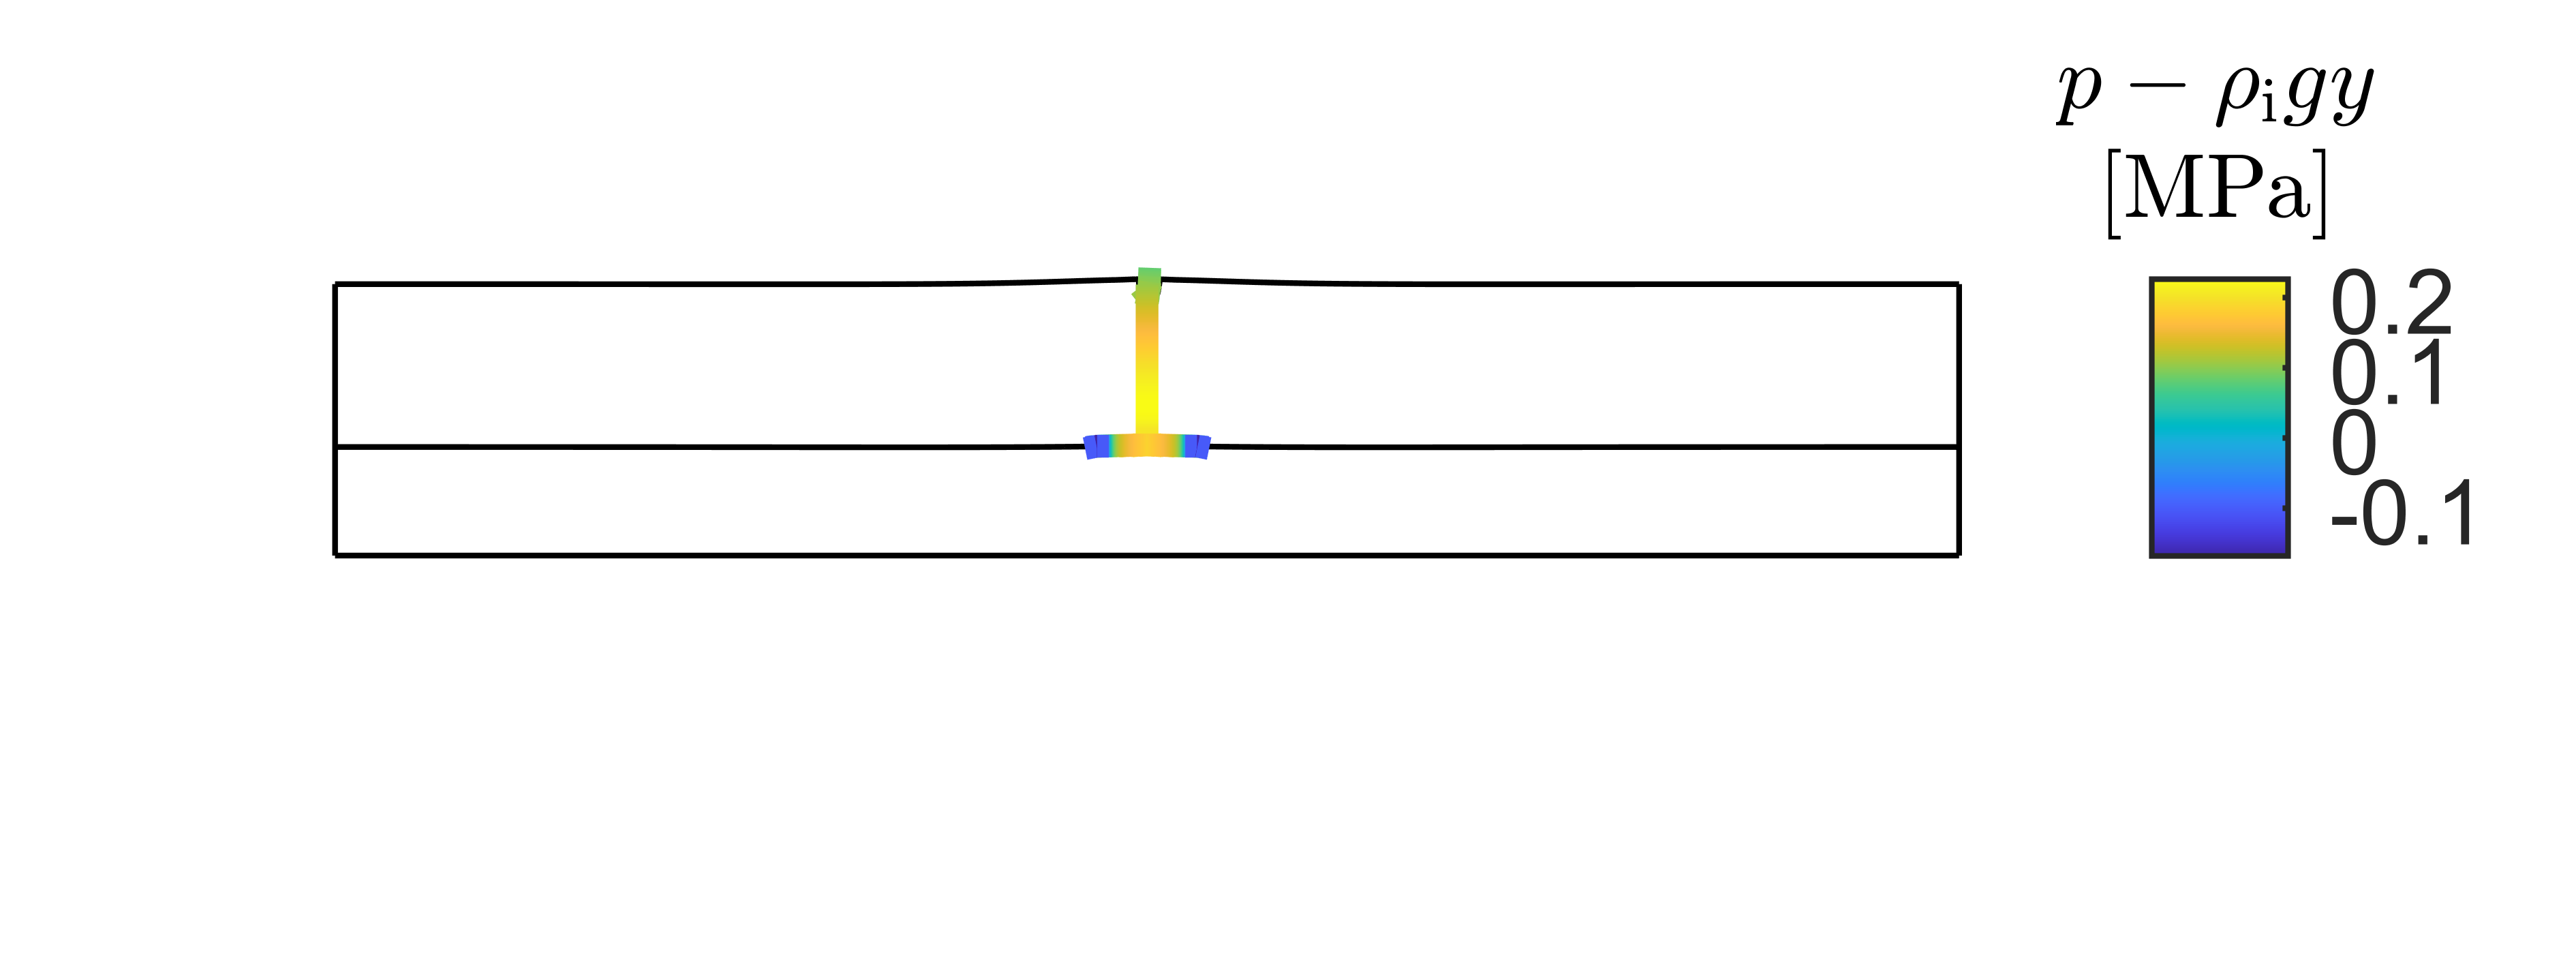
\includegraphics{../Figures/PSurf.png}
         \caption{Pressure and displacements}
         \label{fig:1}
     \end{subfigure}
     \begin{subfigure}[b]{8cm}
         \centering
         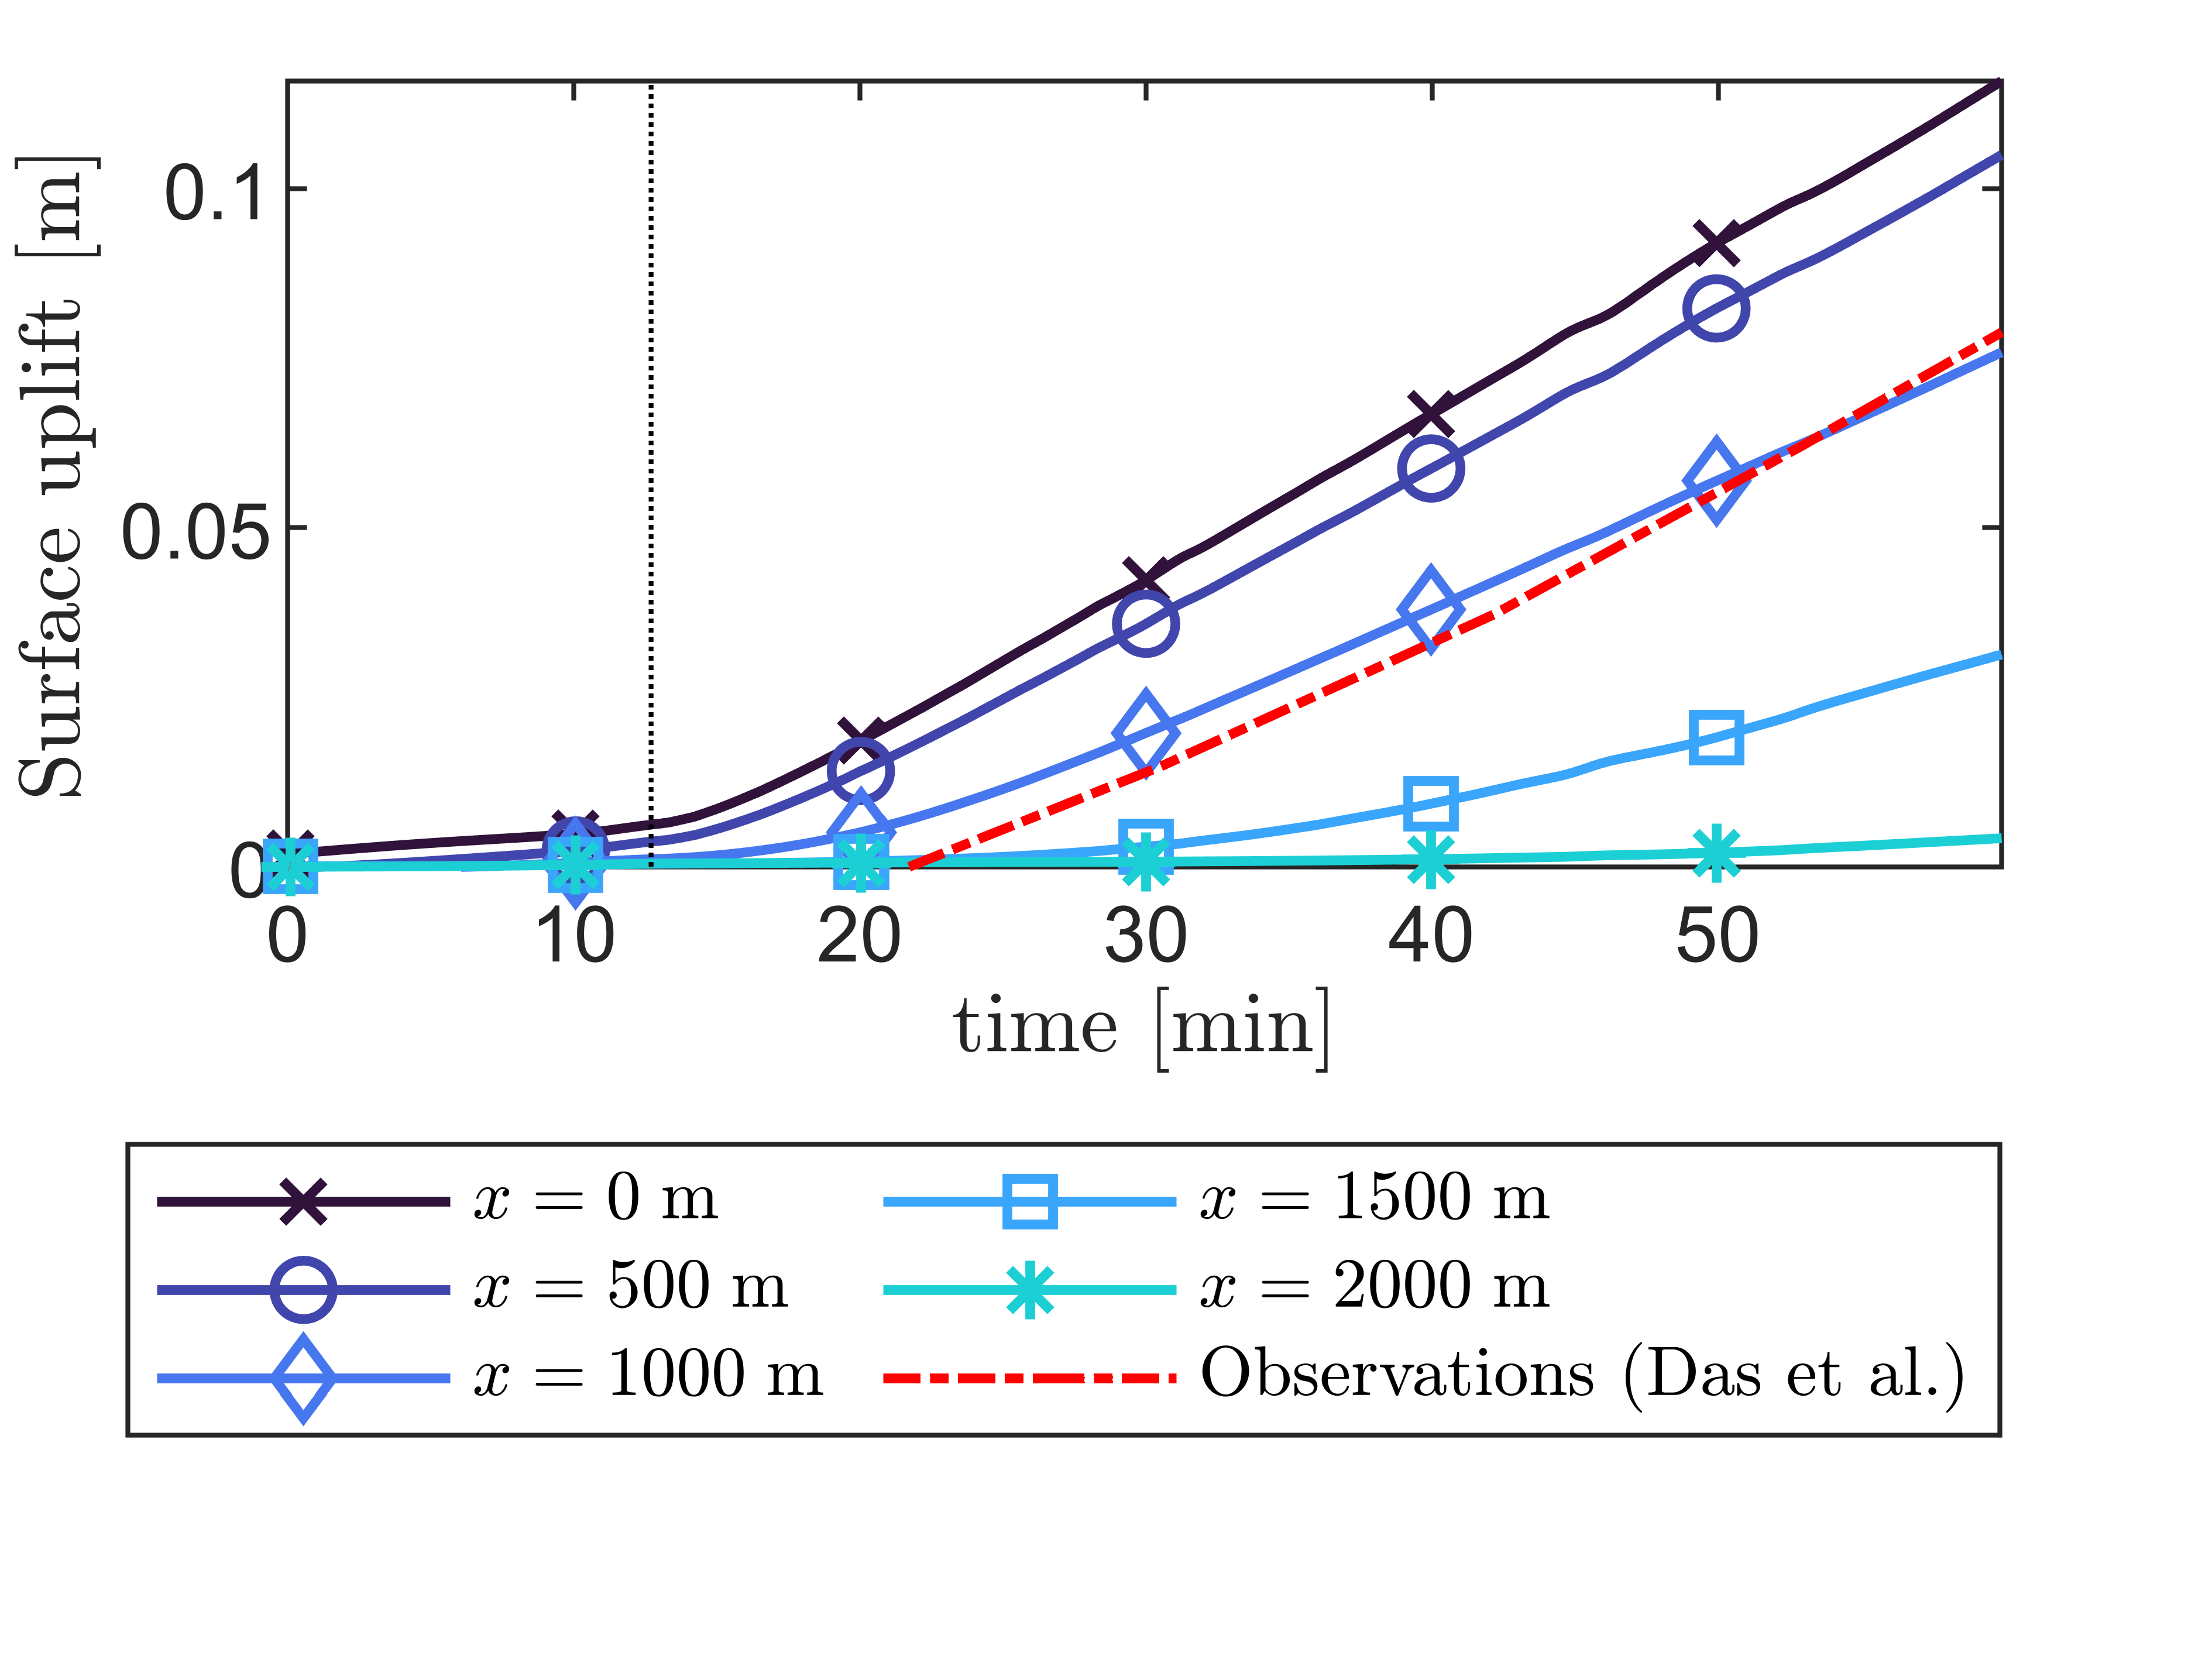
\includegraphics{../Figures/Uplift.png}
         \caption{Vertical displacement}
         \label{fig:2}
     \end{subfigure}
     \begin{subfigure}[b]{8cm}
         \centering
         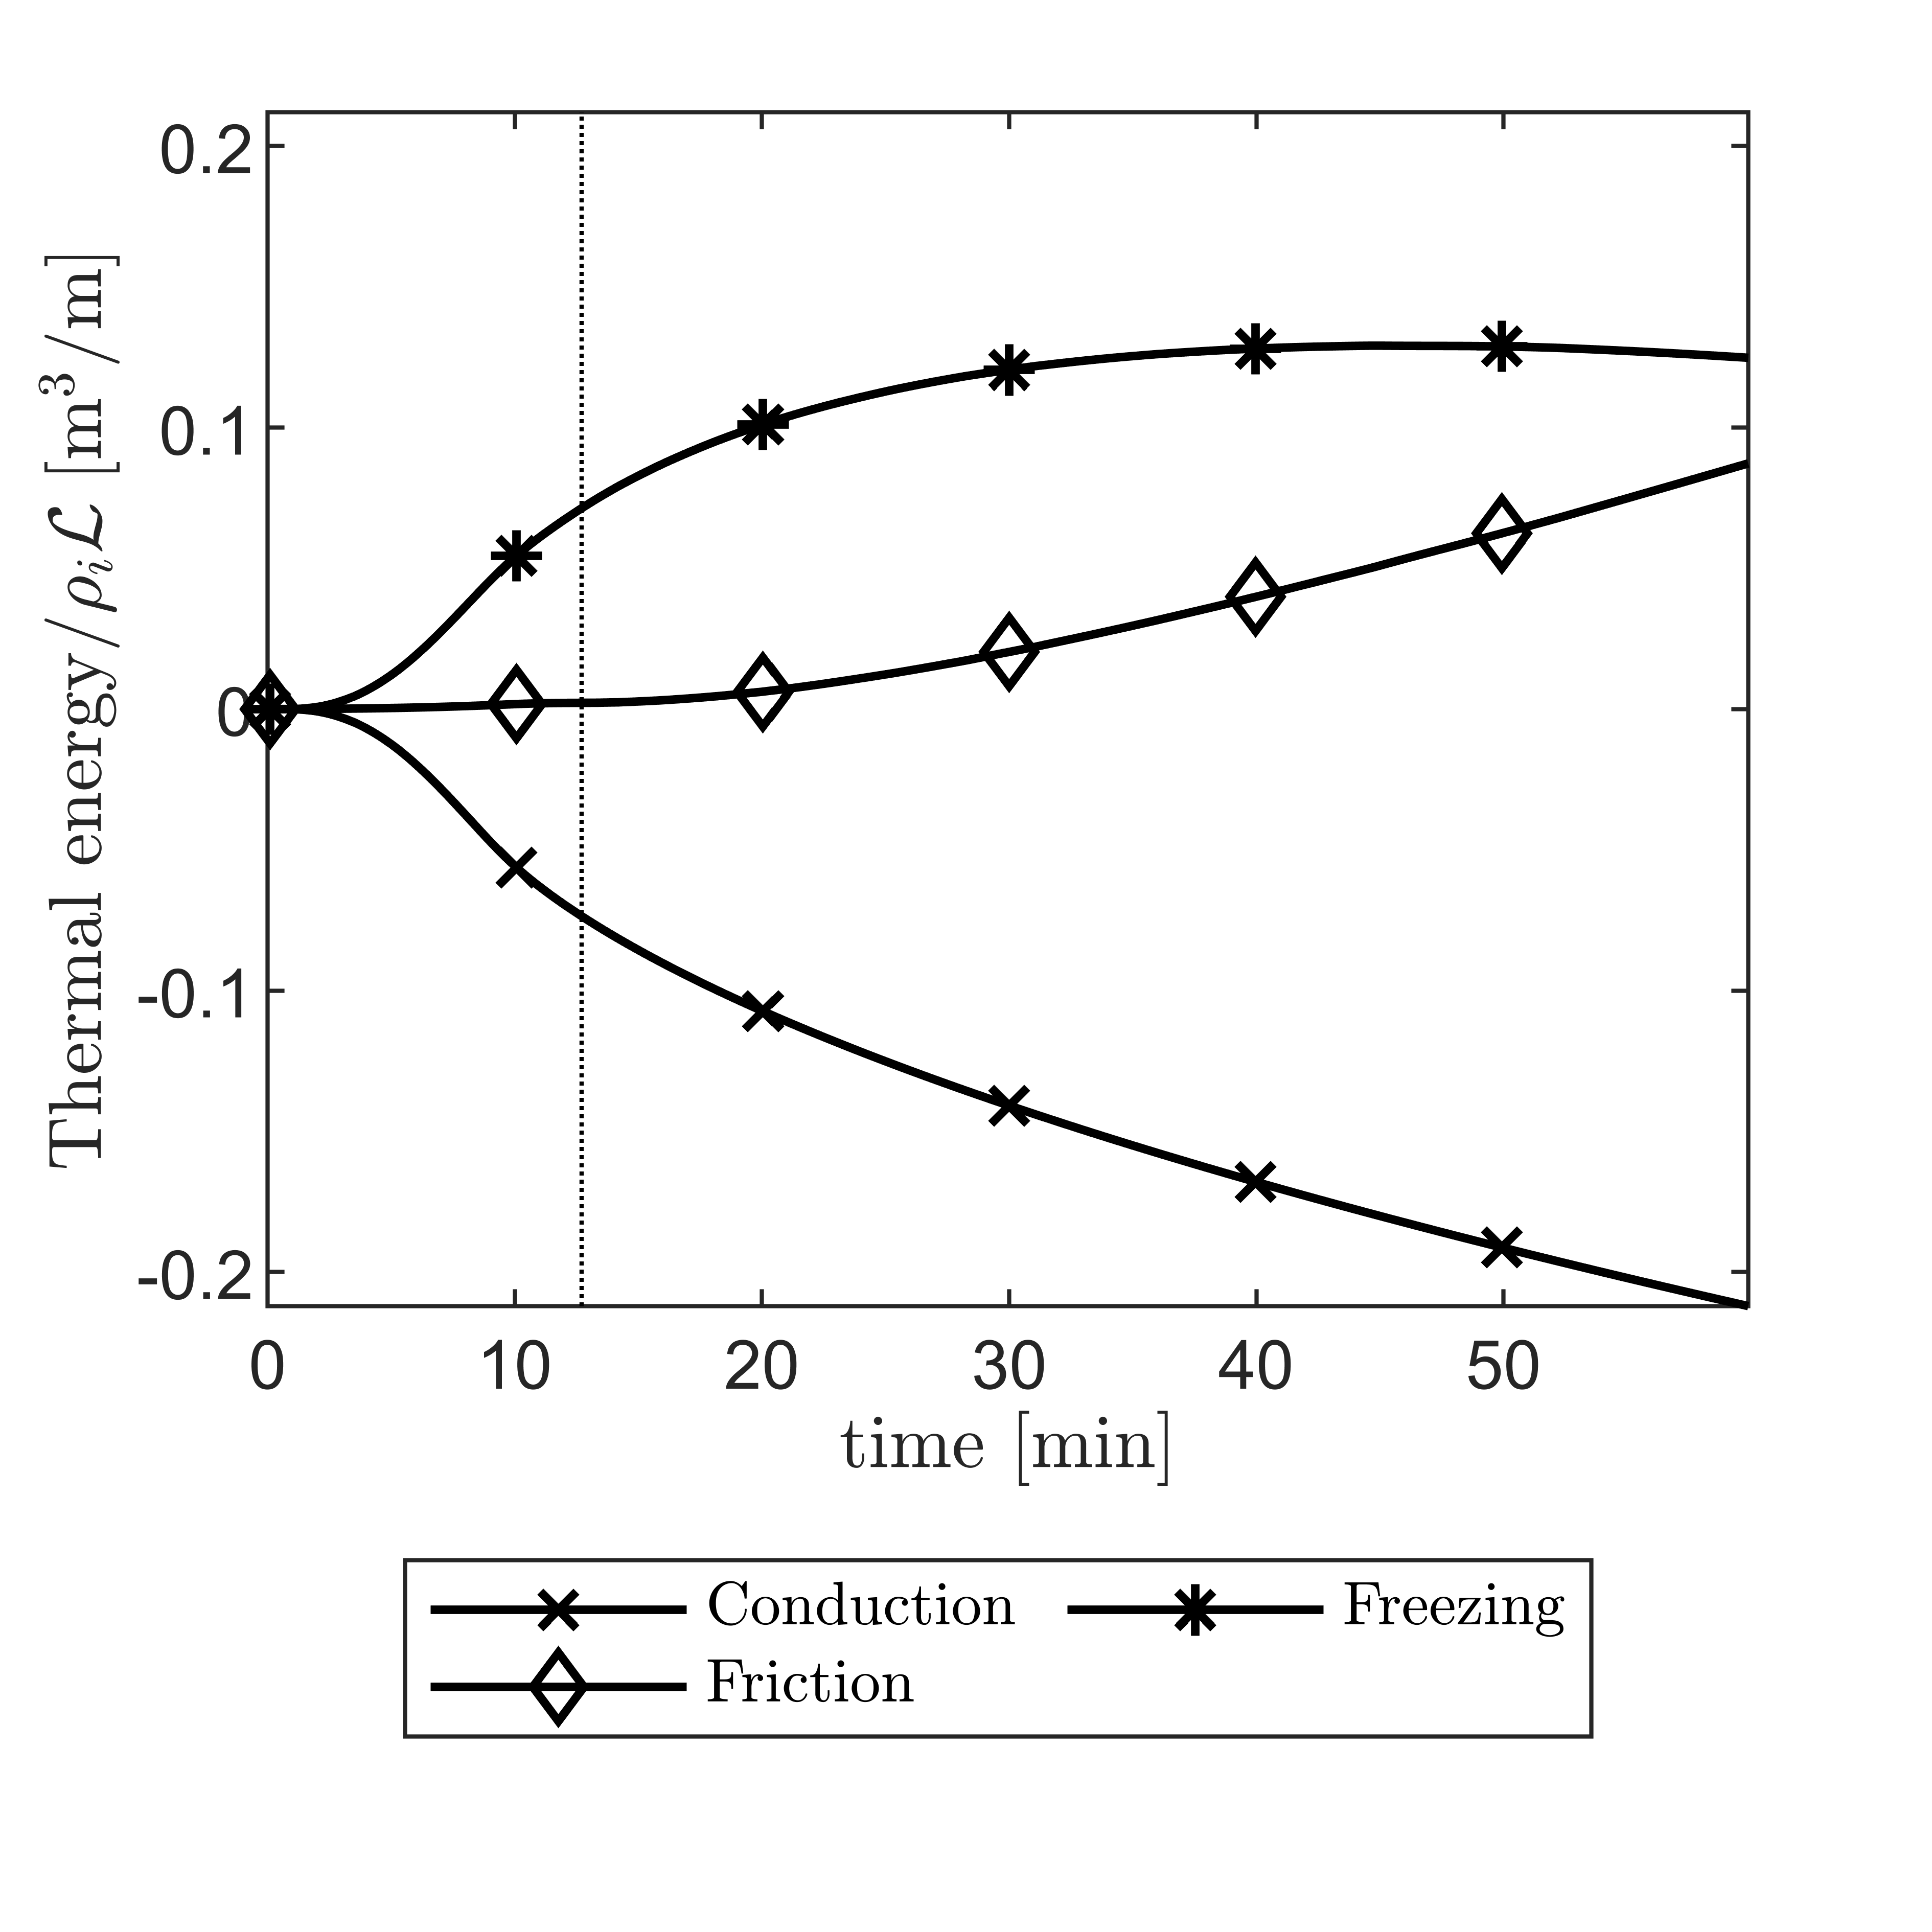
\includegraphics{../Figures/Thermals.png}
         \caption{Thermal energy produced by friction, consumed by conduction, and the resulting effect on freezing}
         \label{fig:3}
     \end{subfigure}
     \begin{subfigure}[b]{8cm}
         \centering
         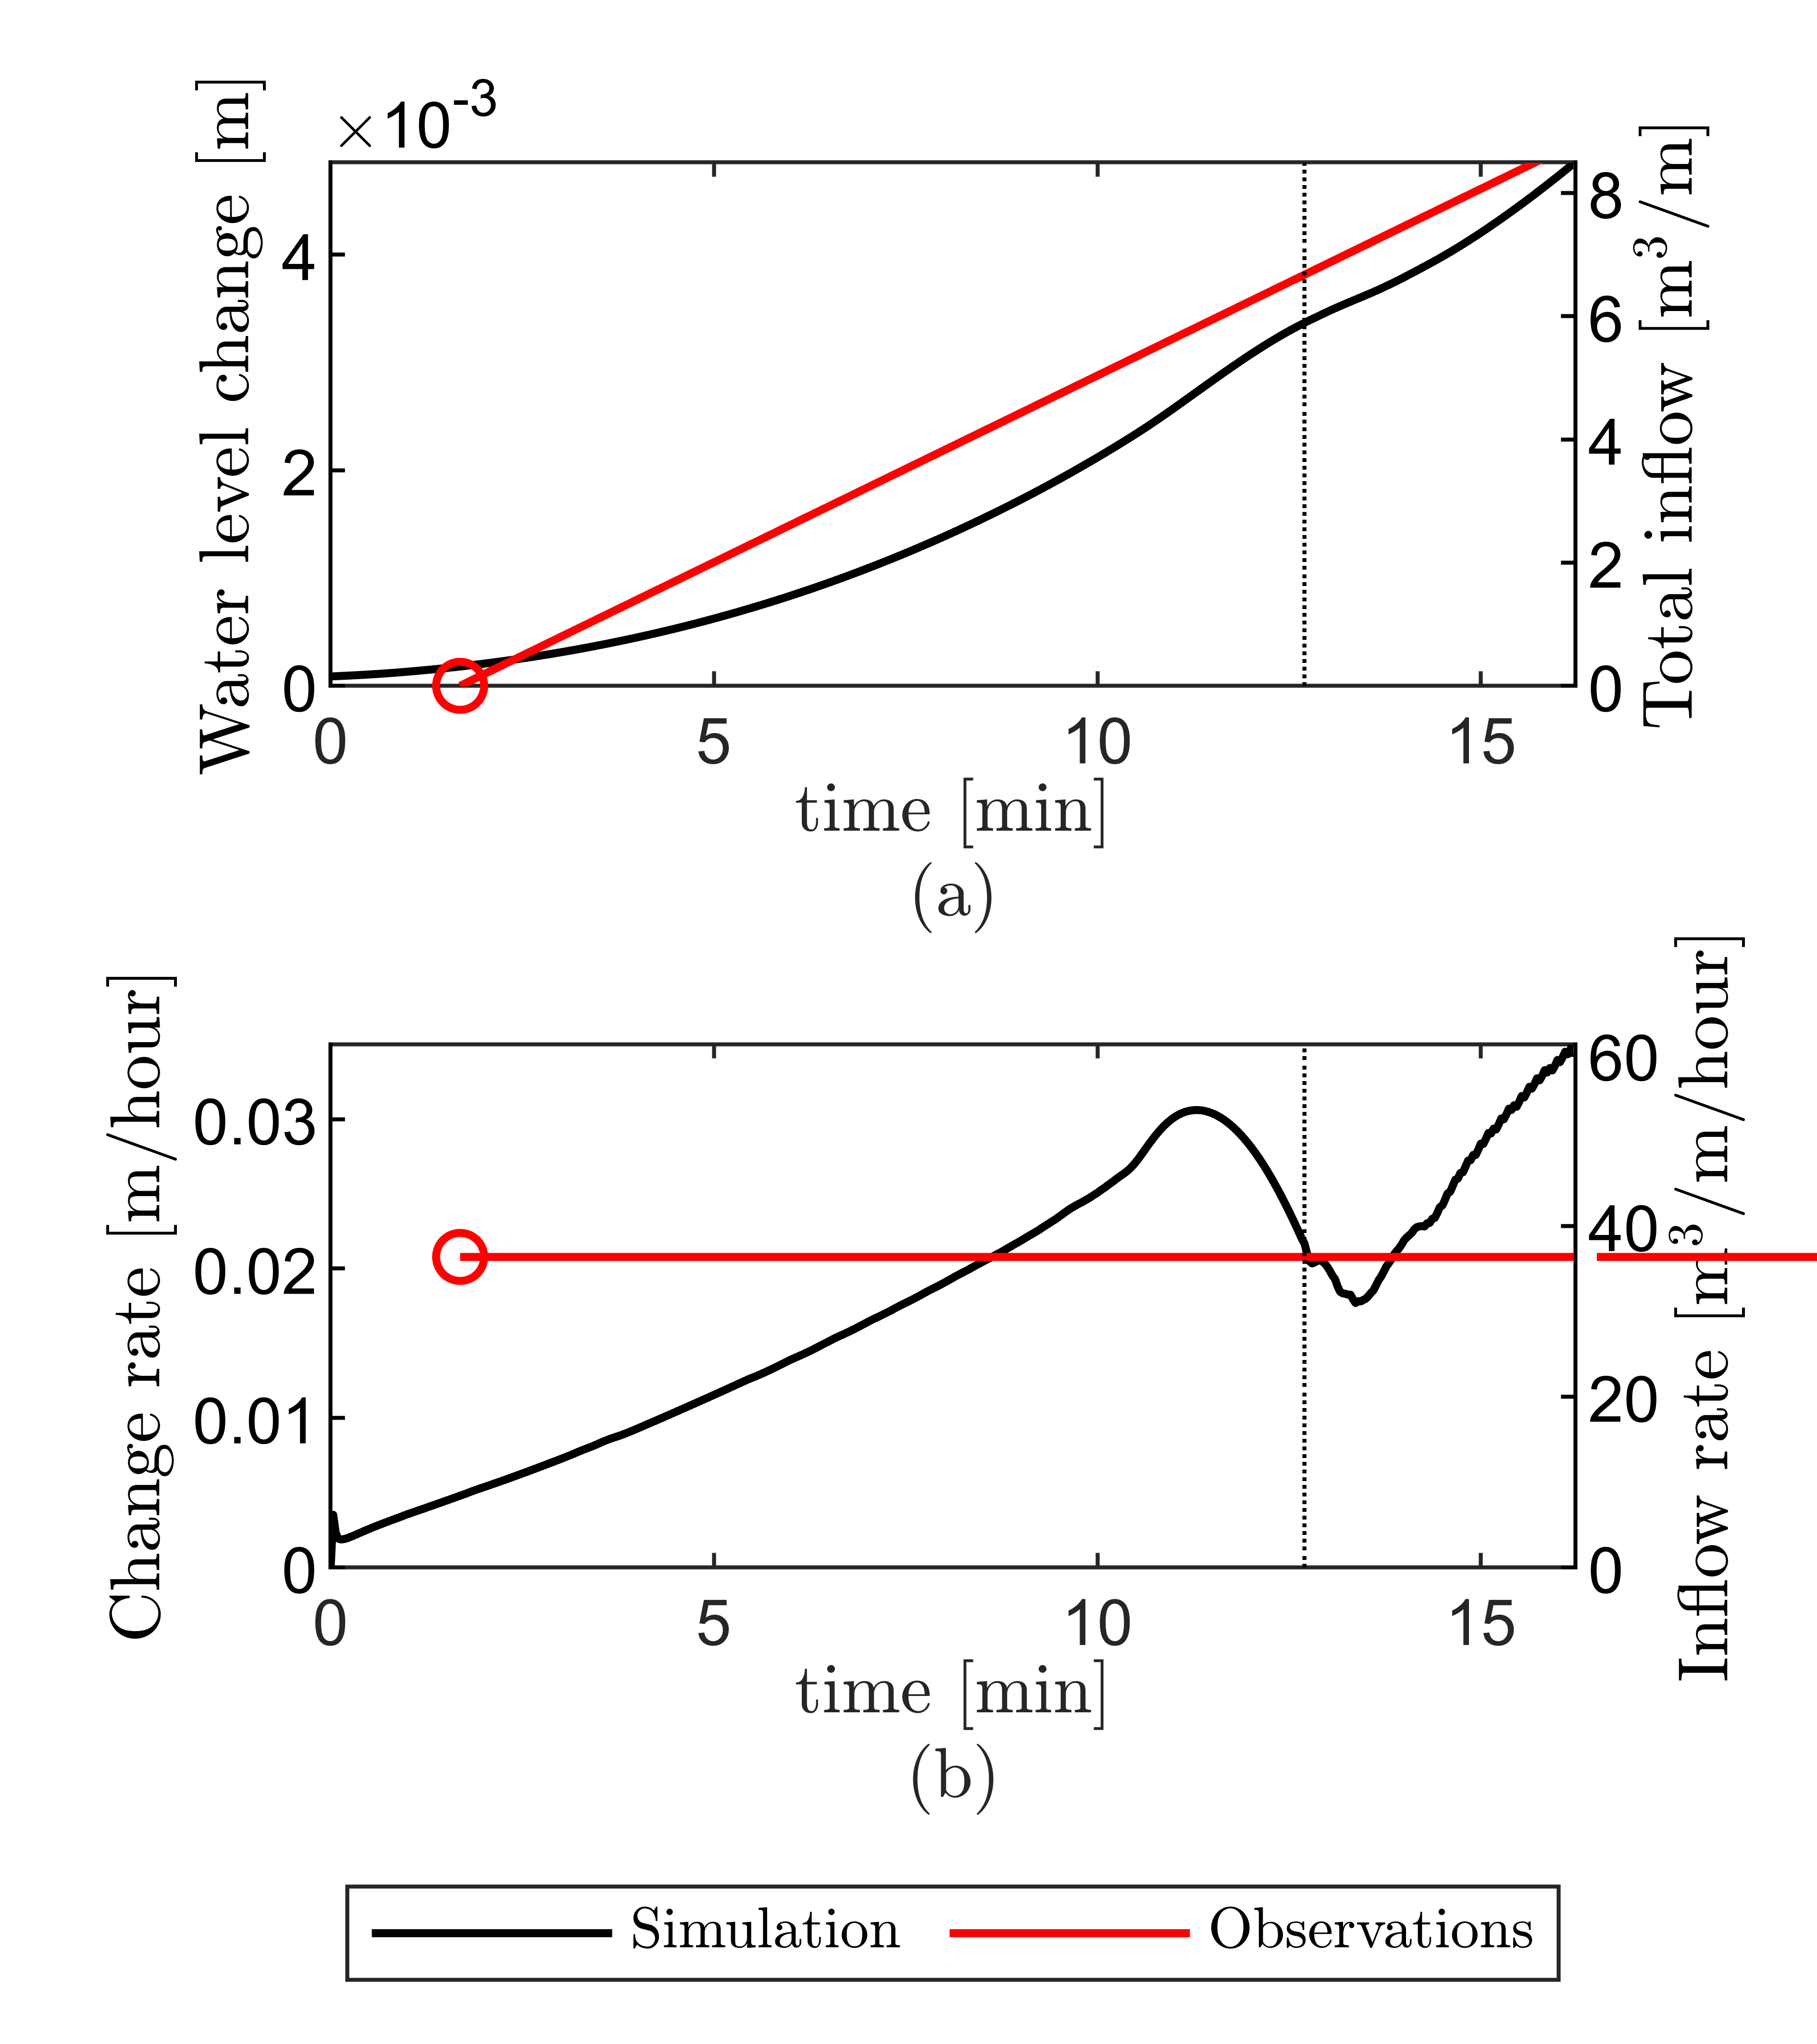
\includegraphics{../Figures/FluidFluxes.png}
         \caption{Water inflow into the crevasse (a), and rate of water inflow (b)}
         \label{fig:4}
     \end{subfigure}
     \begin{subfigure}[b]{8cm}
         \centering
         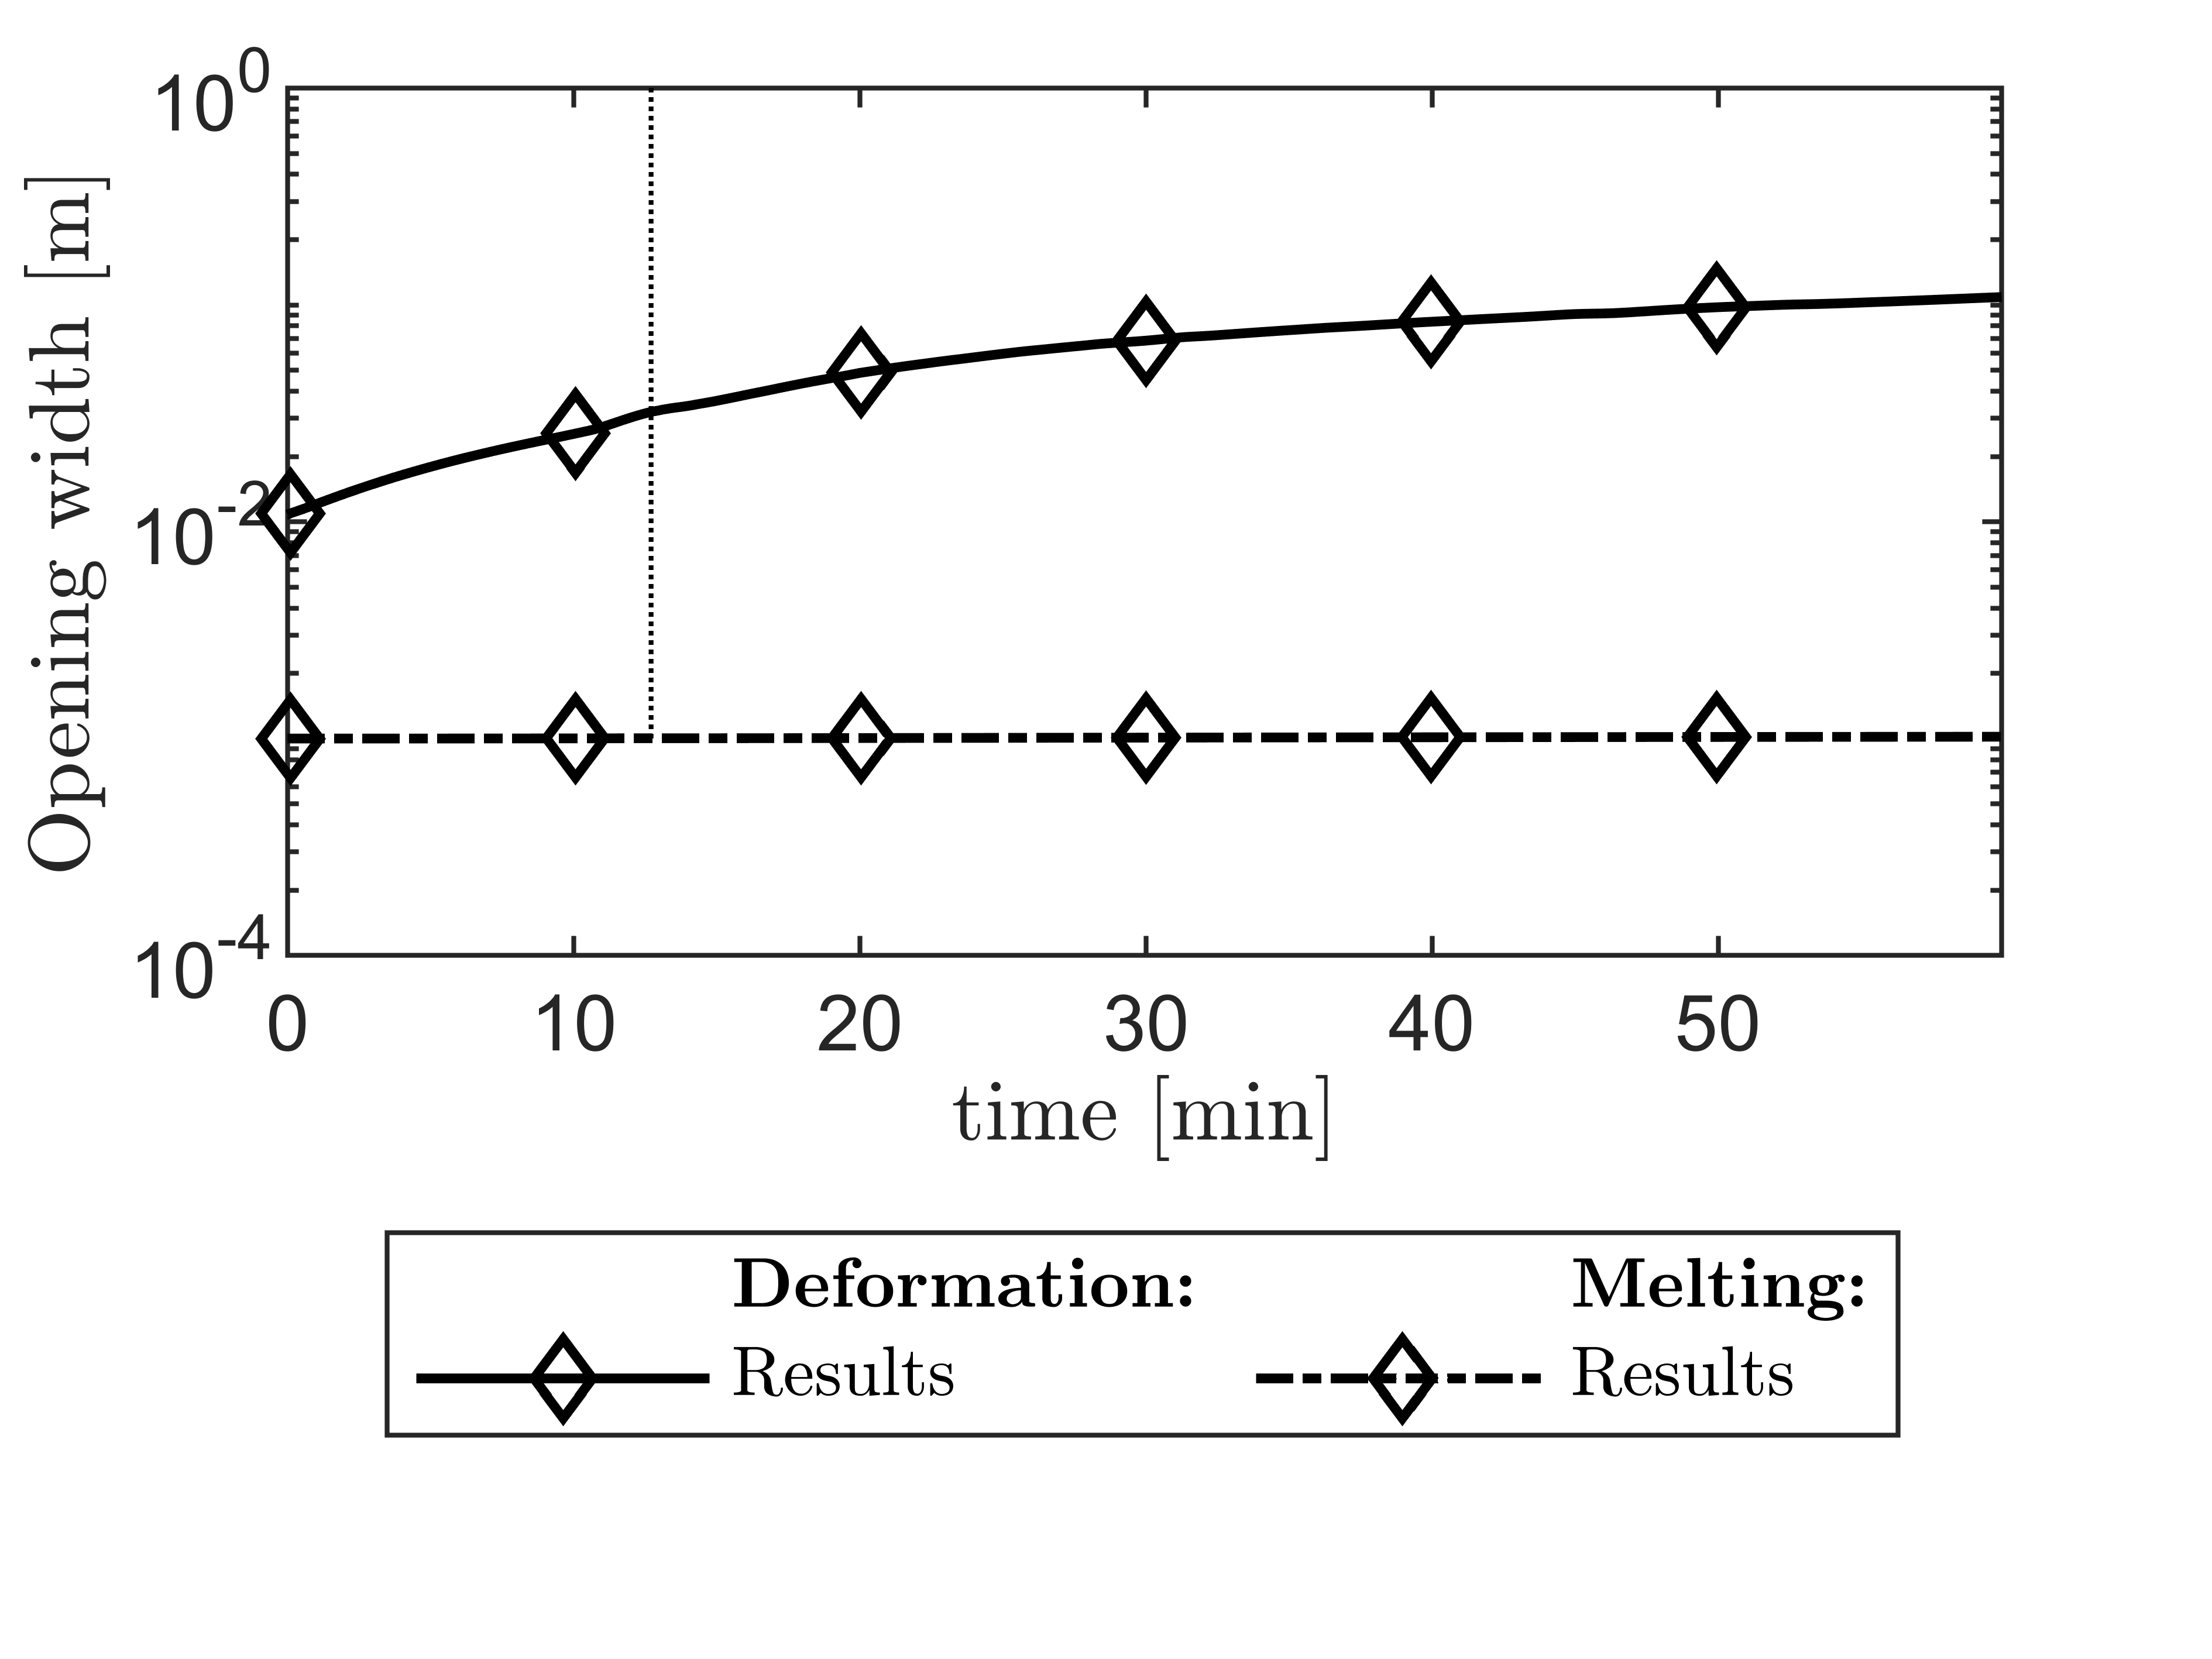
\includegraphics{../Figures/OpeningHeights.png}
         \caption{Mechanical and melting induced crevasse opening heights}
         \label{fig:5}
     \end{subfigure}
     \begin{subfigure}[b]{8cm}
         \centering
         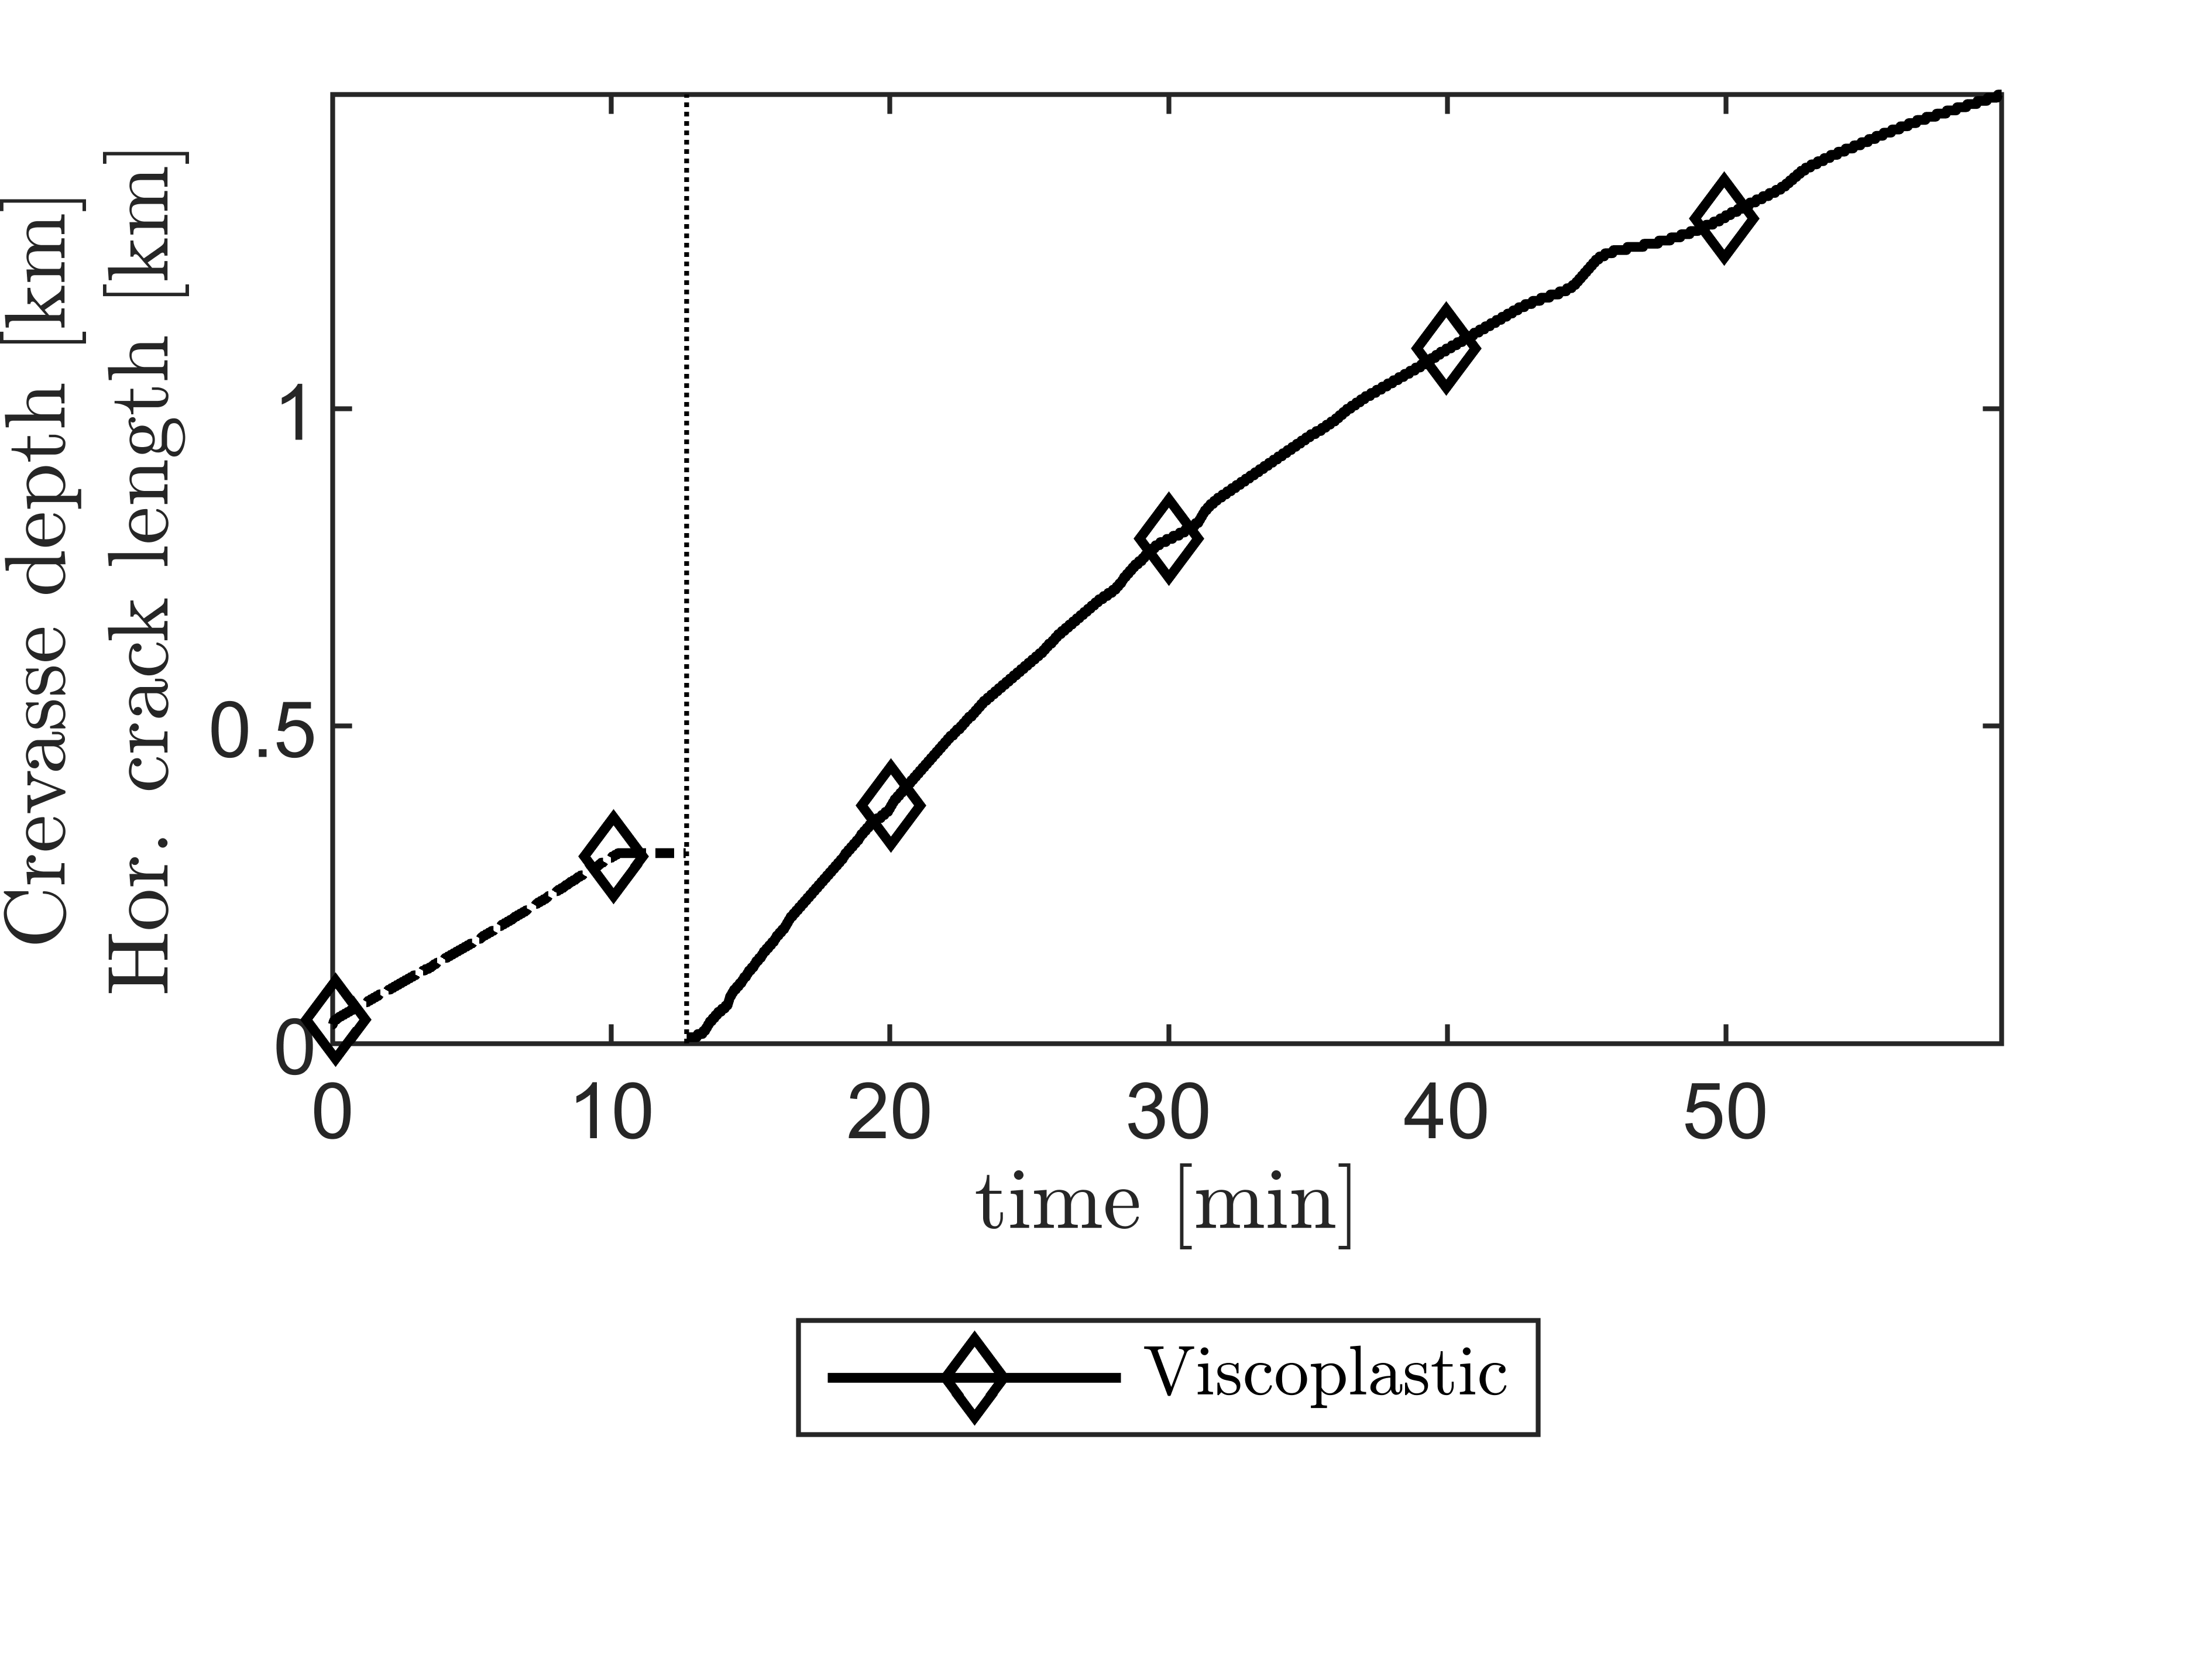
\includegraphics{../Figures/FractureLengths.png}
         \caption{Crevasse depth/vertical crack length}
         \label{fig:6}
     \end{subfigure}
     \caption{Generated figures during postprocessing}
     \label{fig:results}
\end{figure}

Due to the long duration of full ice-sheet simulations, the code is set up to use a smaller geometry as example case. However, both mesh files are included, and this can be switched by referring to Meshes/mesh\_ Das\_ 25.mphtxt as input, using the 980 m thick geometry used for comparison with observations from Das et al. \citep{Das2008}. While the code is running, some results will be plotted, and outputs for post-processing will be saved every 10 time steps to the Results folder. 

The matlab script Postprocessing.m can perform visualisation of these output files. this script requires the name of an output file:
\lstinputlisting[firstnumber=9,firstline=9,lastline=11,style=mystyle,title=PostProcessing.m]{../PostProcessing.m}
it also requires an output file from the end of the initialization time, which is used to define the relative displacements that have occurred during the actual crevasse propagation. To facilitate describing the post-processing preocedure, two output files are included: Reference\_ 150.mat, containing results just before the end of the initialization period, and Results\_ 1950.mat, having results after 1 hour of simulated time (approx. 1 day of running at 8 cpu cores required). 

Within this file, the deformation of the ice-sheet and pressures within the crack, see \cref{fig:1}, are produced via the function:
\lstinputlisting[firstnumber=309,firstline=309,lastline=309,style=mystyle]{../PostProcessing.m}
using the state of the system, saved within the physics objects, a deformation scale sc with with the shown displacements are enhanced, and allowing for the ice to be either filled in (white for ice, grey for rock), or for this to be left transparent (much faster). 

Within the output file, surface displacements are saved for convenient plotting, and can be plotted at several locations as:
\lstinputlisting[firstnumber=56,firstline=56,lastline=60,style=mystyle]{../PostProcessing.m}
Producing figure \cref{fig:2}.
In a similar manner, the total thermal energy lost into the ice due to conduction, produced due to friction, and used to freeze the crevasse walls are plotted (See \cref{fig:3}):
\lstinputlisting[firstnumber=78,firstline=78,lastline=89,style=mystyle]{../PostProcessing.m}
which also uses the script plotsparsemarkers \citep{SparseMarkers} to plot evenly spaced markers that do not correspond to all data points (which are saved every 2 seconds). Flow rates are plotted similarly, \cref{fig:4}:
\lstinputlisting[firstnumber=113,firstline=113,lastline=113,style=mystyle]{../PostProcessing.m}
\lstinputlisting[firstnumber=141,firstline=141,lastline=141,style=mystyle]{../PostProcessing.m}
using data extracted from \citep{Das2008} as reference via the function:
\lstinputlisting[firstnumber=235,firstline=235,lastline=235,style=mystyle]{../PostProcessing.m}
Finally, crevasse opening height, \cref{fig:5}, and crack lengths, \cref{fig:6} as:
\lstinputlisting[firstnumber=176,firstline=176,lastline=176,style=mystyle]{../PostProcessing.m}
\lstinputlisting[firstnumber=195,firstline=195,lastline=201,style=mystyle]{../PostProcessing.m}





\section{References}
\renewcommand{\bibsection}{}
\bibliography{references}

\end{document}
